\documentclass[11pt,a4paper]{article}

% ===================== Codificación y fuentes =====================
\usepackage[utf8]{inputenc}
\usepackage[T1]{fontenc}

% ===================== Página y utilidades ========================
\usepackage[left=2.5cm,right=2.5cm,top=2.5cm,bottom=2.5cm]{geometry}
\usepackage{array}
\usepackage{enumitem}
\usepackage{graphicx}
\usepackage{xcolor}
\usepackage{titlesec}
\usepackage{fancyhdr}
\usepackage[most]{tcolorbox}
\usepackage{hyperref}
\usepackage{booktabs}
\usepackage{float}

% ===================== Etiquetas en español =======================
\renewcommand{\contentsname}{Índice}
\renewcommand{\figurename}{Figura}
\renewcommand{\tablename}{Tabla}
\renewcommand{\refname}{Referencias}

% ===================== Escala de grises ===========================
\definecolor{negro}{RGB}{0,0,0}
\definecolor{gris}{RGB}{90,90,90}
\definecolor{grisclaro}{RGB}{150,150,150}

% ===================== Hipervínculos ===============================
\hypersetup{
  colorlinks=true,
  linkcolor=negro,
  urlcolor=negro,
  citecolor=negro,
  hypertexnames=false,
  pdftitle={Evaluación Formativa 1 - Framingham},
  pdfauthor={Alexander Sepúlveda Ormazábal}
}

% ===================== Estilo de títulos ===========================
\titleformat{\section}{\large\bfseries\color{negro}}{\thesection.}{0.5em}{}
\titleformat{\subsection}{\normalsize\bfseries\color{negro}}{\thesubsection}{0.5em}{}
\titlespacing*{\section}{0pt}{1.4em}{0.4em}
\titlespacing*{\subsection}{0pt}{1.0em}{0.3em}

% ===================== Pie de página ===============================
\pagestyle{fancy}
\fancyhf{}
\fancyfoot[L]{\footnotesize\color{gris}Magíster en Ciencia de Datos e Inteligencia Artificial}
\fancyfoot[R]{\footnotesize\color{gris}\thepage}
\renewcommand{\headrulewidth}{0pt}
\renewcommand{\footrulewidth}{0.4pt}
\setlength{\headheight}{14pt}

% ===================== Cajas de la plantilla =======================
\newtcolorbox{infobox}[1][Información de la evaluación]{
  colback=black!3,
  colframe=negro,
  fonttitle=\bfseries,
  coltitle=white,
  title={#1},
  boxrule=0.6pt,
  arc=1pt,
  left=8pt,
  right=8pt,
  top=6pt,
  bottom=6pt,
  breakable
}

% ===================== Datos del estudiante ========================
\newcommand{\proyTitulo}{Análisis estadístico del riesgo de enfermedad coronaria a diez años}
\newcommand{\proyIntegrantes}{Alexander Sepúlveda Ormazábal}
\newcommand{\proyDataset}{Framingham Heart Study}
\newcommand{\proyDocente}{Jean Paul Maidana González}
\newcommand{\proyFecha}{14/10/2026}
\newcommand{\proyRepo}{\url{https://github.com/alexander-seor/MCDI501-Proyecto-Framingham}}

\setlength{\parindent}{0pt}
\setlength{\parskip}{0.45em}
\setlength{\emergencystretch}{2em}
\setlist[itemize]{leftmargin=1.4em,itemsep=0.2em,topsep=0.3em}

\begin{document}
\pagenumbering{gobble}

% ===================== Portada =====================================
\thispagestyle{empty}
\begin{center}
\vspace*{0.8cm}

\includegraphics[height=4.2cm]{logo_unab.png}\\[1.1cm]

{\footnotesize\color{gris}\MakeUppercase{Magíster en Ciencia de Datos e Inteligencia Artificial}}\\[0.15cm]
{\footnotesize\color{grisclaro}MCDI501: Estadística Computacional para la Toma de Decisiones}\\[1.7cm]

{\Large\bfseries\color{negro}Evaluación Formativa 1}\\[0.4cm]
{\large\color{negro}Análisis Exploratorio e Inferencial (práctica)}\\[0.9cm]

{\small\itshape\color{gris}Informe individual \textperiodcentered\ 0\,\% (formativa)}
\end{center}

\vspace{1.3cm}

\begin{flushleft}
\newcommand{\datodeportada}[2]{%
  \noindent
  \begin{minipage}[t]{4.0cm}\vspace{0pt}\bfseries\color{negro}#1\end{minipage}%
  \hspace{0.5cm}%
  \begin{minipage}[t]{10.8cm}\vspace{0pt}#2\end{minipage}%
  \par\vspace{0.55em}%
}
\datodeportada{Título del proyecto:}{\proyTitulo}
\datodeportada{Estudiante:}{\proyIntegrantes}
\datodeportada{Dataset:}{\proyDataset}
\datodeportada{Docente:}{\proyDocente}
\datodeportada{Fecha:}{\proyFecha}
\datodeportada{Repositorio GitHub:}{\proyRepo}
\end{flushleft}

\clearpage
\pagenumbering{arabic}

\begin{infobox}
\textbf{Fase del proyecto:} Fase 1: Definición y orientación de la situación del proyecto\\
\textbf{Modalidad:} Individual\qquad\textbf{Ponderación:} 0\,\% (formativa)\\
\textbf{Entregable:} Informe en formato PDF, subido a Canvas\\
\textbf{Resultado de aprendizaje (RA1):} aplicar conceptos fundamentales de probabilidad e inferencia estadística en la resolución de problemas de decisión bajo incertidumbre.\\
\textbf{Indicadores evaluados:} ID1.2, ID1.3 e ID1.4.
\end{infobox}

\vspace{0.5em}
\tableofcontents
\newpage

% ===================== 1. Introducción =============================
% Guía oficial de la plantilla:
% Presenten brevemente el conjunto de datos definido por el equipo en la fase
% anterior del proyecto y el propósito de este informe de avance.
\section{Introducción}

Las enfermedades cardiovasculares constituyen un problema relevante de salud pública y su aparición se relaciona con una combinación de características demográficas, conductuales y clínicas. En este contexto, el proyecto utiliza una versión del conjunto de datos del \textit{Framingham Heart Study}, obtenida desde Kaggle \cite{dileep} y documentada con apoyo de los materiales docentes del National Heart, Lung, and Blood Institute \cite{nhlbi}.

La base contiene 4.238 observaciones y 16 variables. Estas incluyen sexo, edad, nivel educacional, tabaquismo, antecedentes médicos, colesterol, presión arterial, índice de masa corporal, frecuencia cardíaca y glucosa. La variable de respuesta, \texttt{TenYearCHD}, indica si la persona desarrolló enfermedad coronaria durante los diez años de seguimiento: 0 representa ausencia del evento y 1 representa su ocurrencia.

El objetivo del informe es caracterizar el conjunto de datos mediante estadística descriptiva, estimar parámetros relevantes con intervalos de confianza y evaluar una diferencia entre grupos mediante una prueba de hipótesis básica. El análisis busca responder la siguiente pregunta:

\begin{quote}
\textit{¿Qué diferencias demográficas, conductuales y clínicas se observan entre las personas que desarrollaron y las que no desarrollaron enfermedad coronaria durante los diez años de seguimiento?}
\end{quote}

Los resultados se interpretan como evidencia descriptiva y asociativa dentro de la población de referencia del estudio. Debido al carácter observacional de los datos, no se formulan conclusiones causales.

% ===================== 2. Descriptiva ==============================
% Guía oficial de la plantilla (15 pts, ID1.2):
% Caractericen las variables mediante medidas de tendencia central, dispersión
% y representaciones gráficas adecuadas a cada tipo de variable.
\section{Aplicación de estadística descriptiva}

\subsection{Estructura, tipos de variables y calidad de los datos}

El conjunto de datos se cargó sin modificar el archivo original. No se detectaron filas duplicadas. Se identificaron datos ausentes en siete variables: \texttt{education} (2,48\,\%), \texttt{cigsPerDay} (0,68\,\%), \texttt{BPMeds} (1,25\,\%), \texttt{totChol} (1,18\,\%), \texttt{BMI} (0,45\,\%), \texttt{heartRate} (0,02\,\%) y \texttt{glucose} (9,16\,\%). En esta etapa no se imputaron valores; cada procedimiento utilizó los registros disponibles para las variables involucradas.

Aunque todas las columnas están almacenadas numéricamente, varias representan categorías. La Tabla~\ref{tab:tipos} resume su clasificación estadística.

\begin{table}[H]
\centering
\caption{Clasificación de las variables del conjunto de datos.}
\label{tab:tipos}
\small
\begin{tabular}{>{\raggedright\arraybackslash}p{2.8cm}>{\raggedright\arraybackslash}p{4.7cm}>{\raggedright\arraybackslash}p{6.7cm}}
\toprule
\textbf{Tipo} & \textbf{Variables} & \textbf{Interpretación} \\
\midrule
Cualitativas nominales dicotómicas & \texttt{male}, \texttt{currentSmoker}, \texttt{BPMeds}, \texttt{prevalentStroke}, \texttt{prevalentHyp}, \texttt{diabetes}, \texttt{TenYearCHD} & Códigos 0 y 1 que representan categorías; no son cantidades sobre las que corresponda calcular promedios. \\
\addlinespace
Cualitativa ordinal & \texttt{education} & Cuatro niveles educacionales ordenados, sin asumir distancias equivalentes entre categorías. \\
\addlinespace
Cuantitativas discretas & \texttt{age}, \texttt{cigsPerDay} & Valores registrados mediante años cumplidos y conteo diario de cigarrillos. \\
\addlinespace
Cuantitativas continuas & \texttt{totChol}, \texttt{sysBP}, \texttt{diaBP}, \texttt{BMI}, \texttt{heartRate}, \texttt{glucose} & Mediciones clínicas expresadas en sus respectivas escalas y unidades. \\
\bottomrule
\end{tabular}
\end{table}

\subsection{Variables cuantitativas}

Para las variables cuantitativas se calcularon tamaño muestral efectivo, media, mediana, desviación estándar y rango intercuartílico (RIC). La Tabla~\ref{tab:descriptiva} muestra que algunas distribuciones son aproximadamente centradas, mientras que otras presentan asimetría o valores extremos. La diferencia entre media y mediana es especialmente visible en cigarrillos por día y glucosa.

\begin{table}[H]
\centering
\caption{Resumen descriptivo de las variables cuantitativas.}
\label{tab:descriptiva}
\small
\begin{tabular}{lrrrrr}
\toprule
\textbf{Variable} & \textbf{$n$} & \textbf{Media} & \textbf{Mediana} & \textbf{DE} & \textbf{RIC} \\
\midrule
Edad (años)                  & 4.238 & 49,58  & 49,00  & 8,57  & 14,00 \\
Cigarrillos por día          & 4.209 & 9,00   & 0,00   & 11,92 & 20,00 \\
Colesterol total (mg/dL)     & 4.188 & 236,72 & 234,00 & 44,59 & 57,00 \\
Presión sistólica (mmHg)     & 4.238 & 132,35 & 128,00 & 22,04 & 27,00 \\
Presión diastólica (mmHg)    & 4.238 & 82,89  & 82,00  & 11,91 & 14,88 \\
Índice de masa corporal      & 4.219 & 25,80  & 25,40  & 4,08  & 4,97  \\
Frecuencia cardíaca (lpm)    & 4.237 & 75,88  & 75,00  & 12,03 & 15,00 \\
Glucosa (mg/dL)              & 3.850 & 81,97  & 78,00  & 23,96 & 16,00 \\
\bottomrule
\end{tabular}
\end{table}

La Figura~\ref{fig:distribuciones} confirma una concentración de \texttt{cigsPerDay} en cero, correspondiente a personas que no fuman, y una cola derecha pronunciada en \texttt{glucose}. También se observan valores elevados en colesterol, presión sistólica e índice de masa corporal. Por esta razón, la media y la desviación estándar se interpretan junto con la mediana y el RIC, menos sensibles a observaciones extremas.

\begin{figure}[H]
\centering
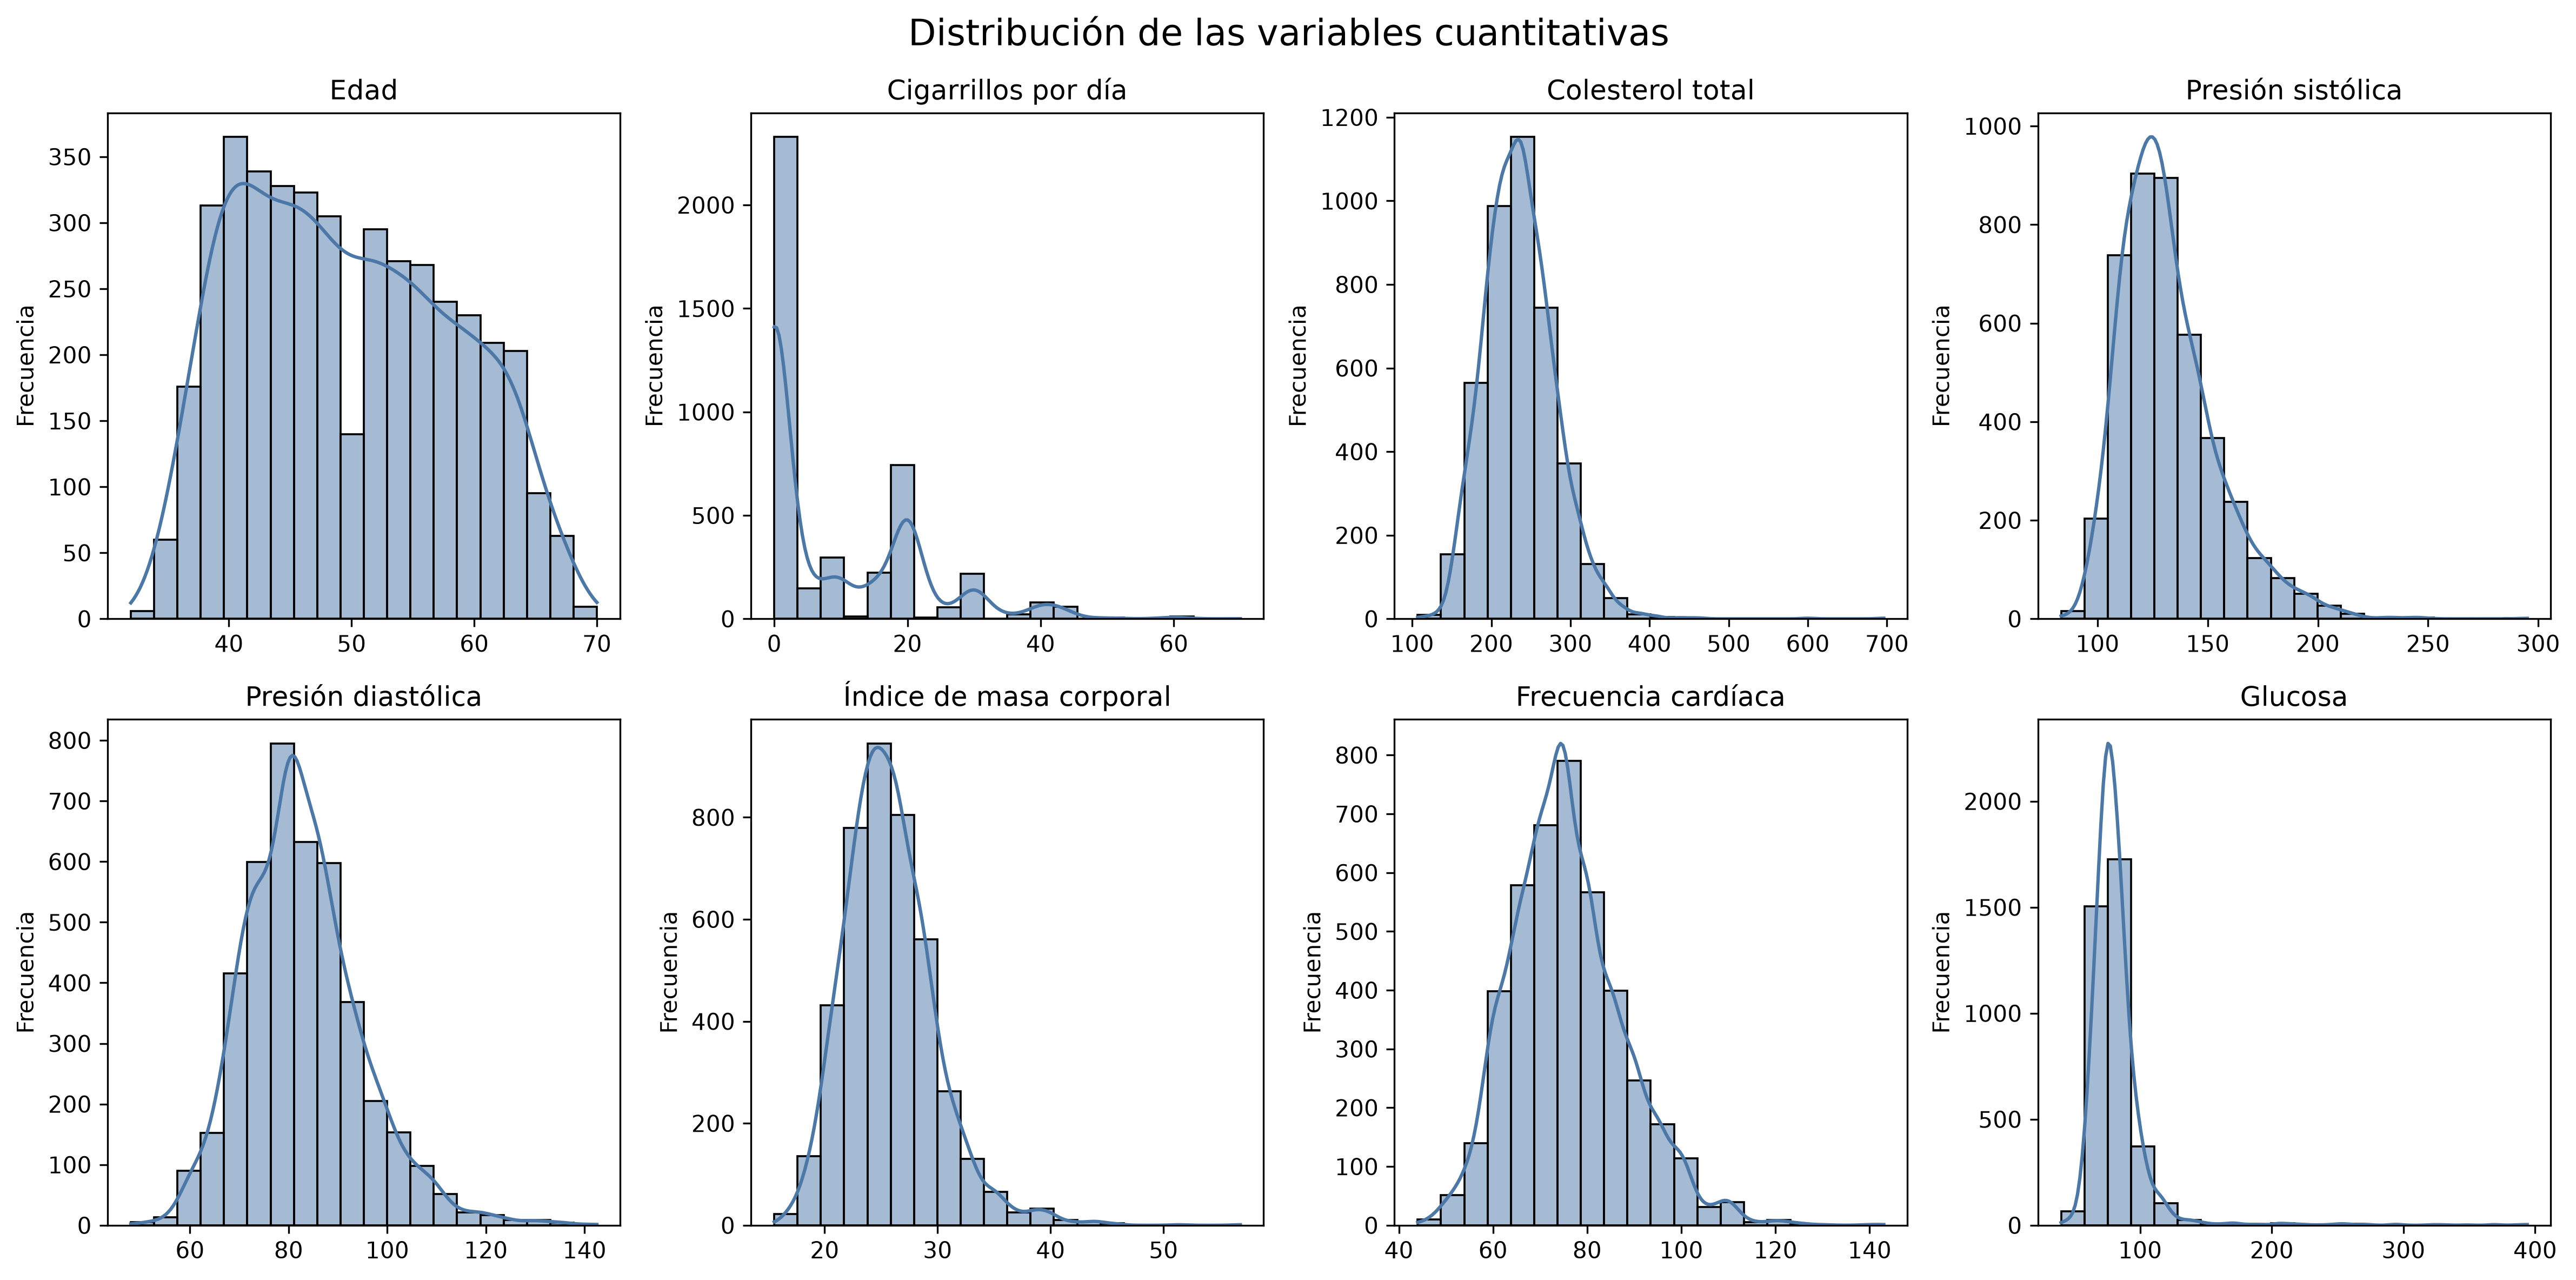
\includegraphics[width=0.98\textwidth]{../figuras/distribuciones_cuantitativas.png}
\caption{Distribución de las variables cuantitativas.}
\label{fig:distribuciones}
\end{figure}

\subsection{Variables categóricas y relaciones preliminares}

La muestra está compuesta por 57,08\,\% de mujeres y 42,92\,\% de hombres. El 49,41\,\% registra tabaquismo actual; 31,05\,\% presenta antecedente de hipertensión y 2,57\,\% tiene diabetes. Respecto del resultado principal, 644 personas desarrollaron enfermedad coronaria, equivalentes al 15,20\,\% de la muestra, mientras que 3.594 no presentaron el evento (84,80\,\%). La Figura~\ref{fig:chd} evidencia el desequilibrio entre ambos grupos.

\begin{figure}[H]
\centering
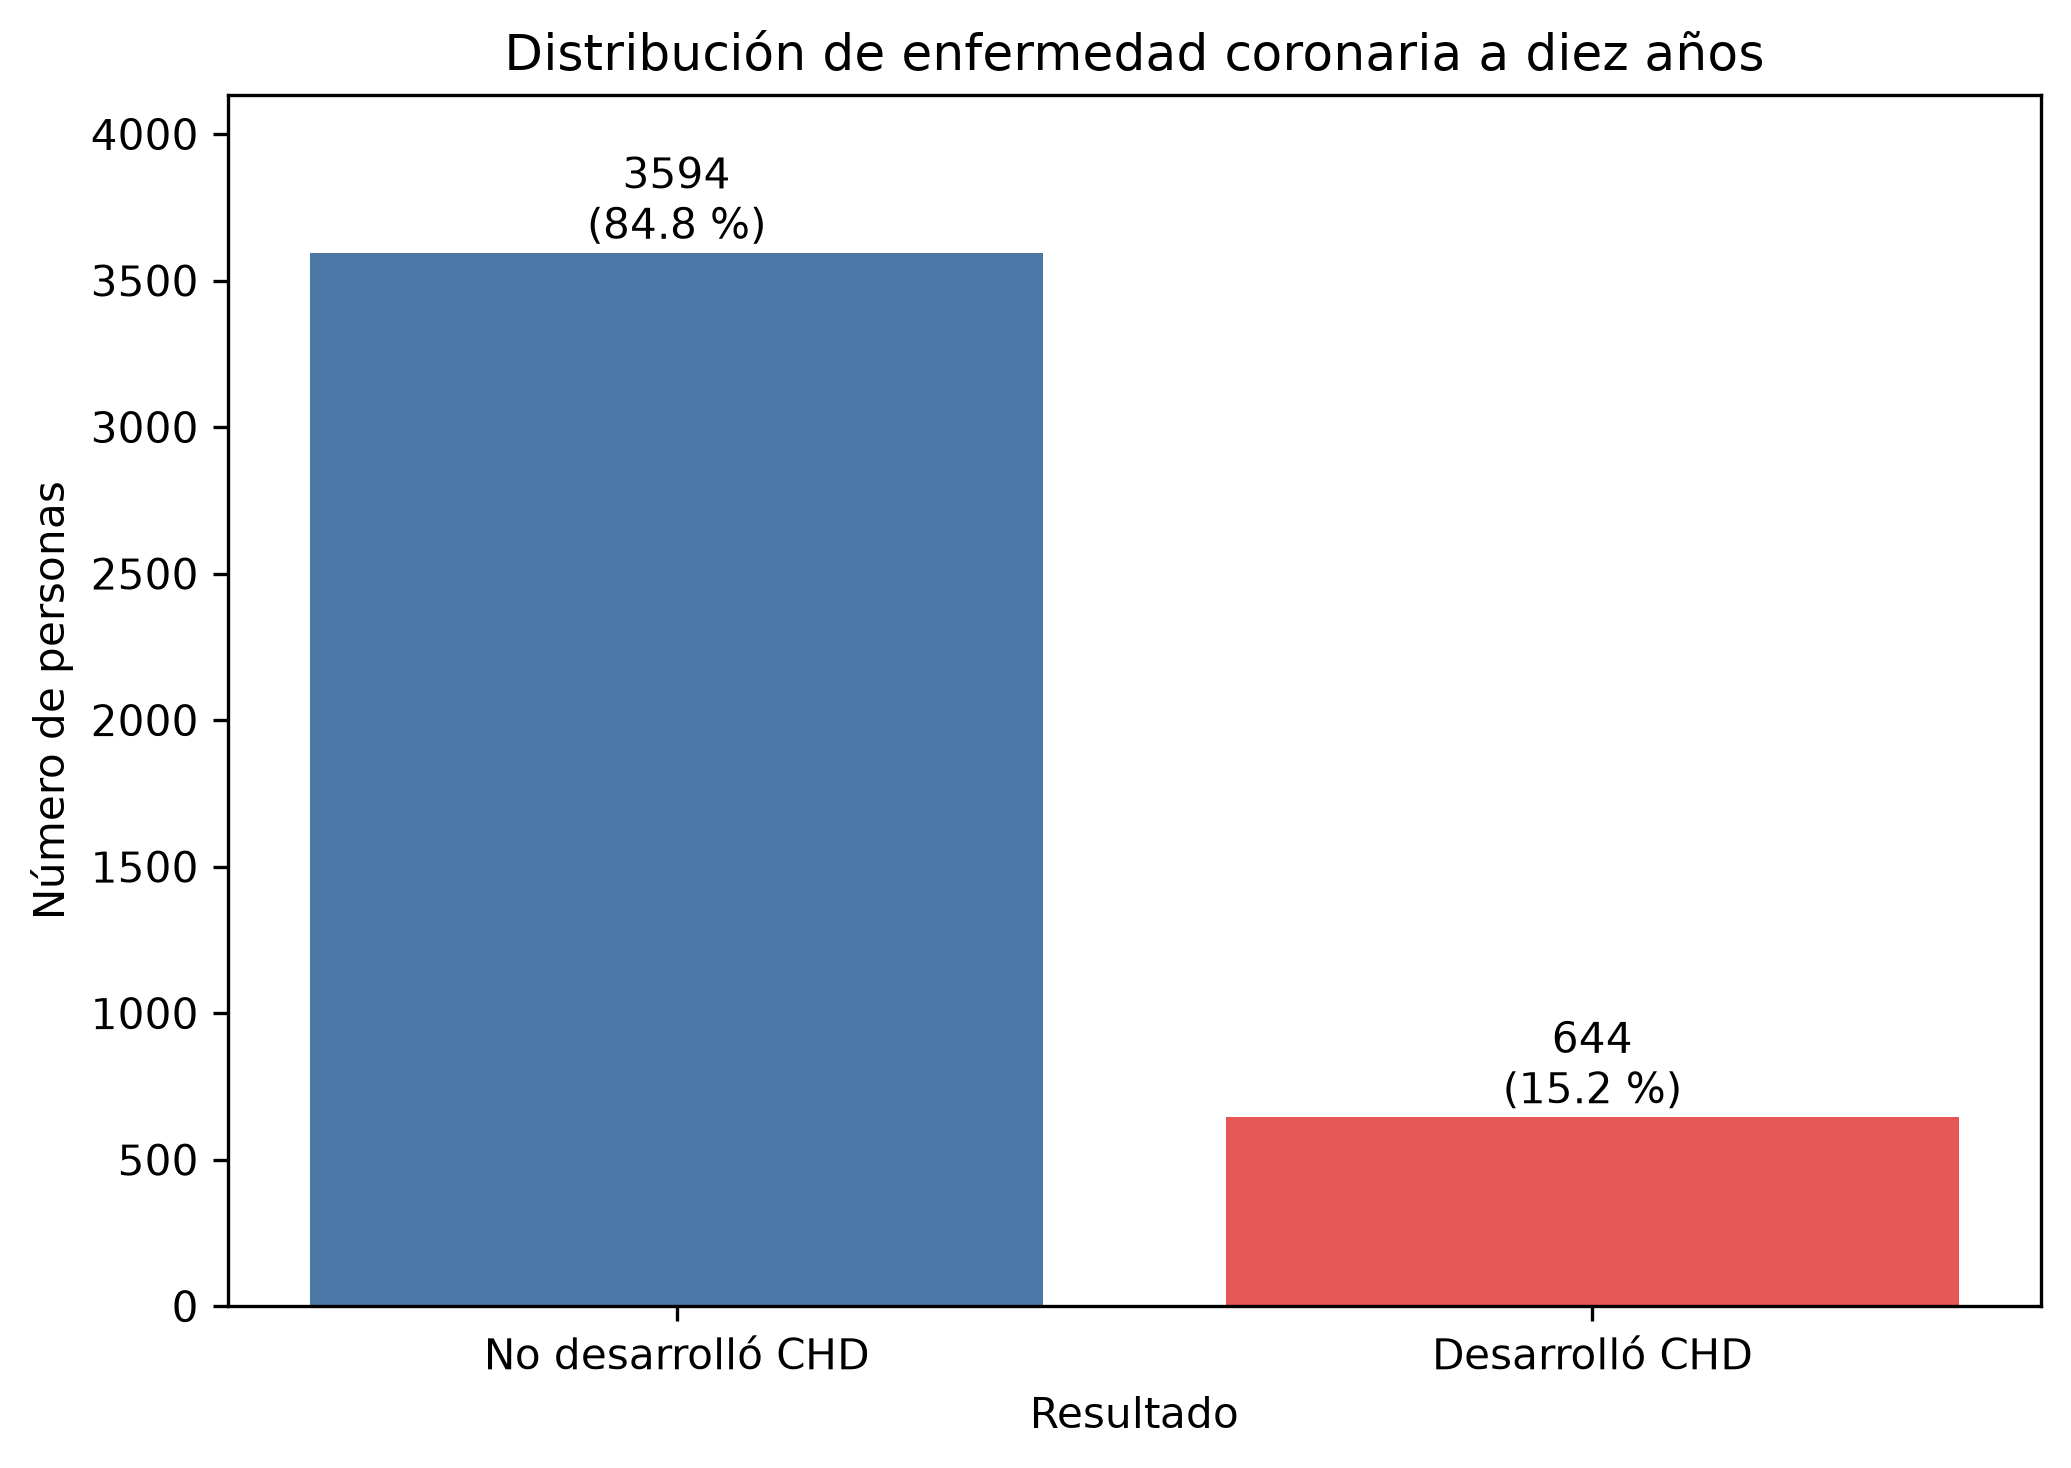
\includegraphics[width=0.65\textwidth]{../figuras/distribucion_chd.png}
\caption{Distribución de enfermedad coronaria durante el seguimiento.}
\label{fig:chd}
\end{figure}

Los diagramas de caja de la Figura~\ref{fig:comparacion} sugieren que las personas que desarrollaron enfermedad coronaria presentan, en general, mayor edad y presión sistólica. Para el índice de masa corporal existe un solapamiento considerable entre grupos. La glucosa exhibe valores extremos y una distribución desplazada hacia valores mayores en el grupo con enfermedad. Estas diferencias son exploratorias y los gráficos, por sí solos, no establecen significancia estadística ni causalidad.

\begin{figure}[H]
\centering
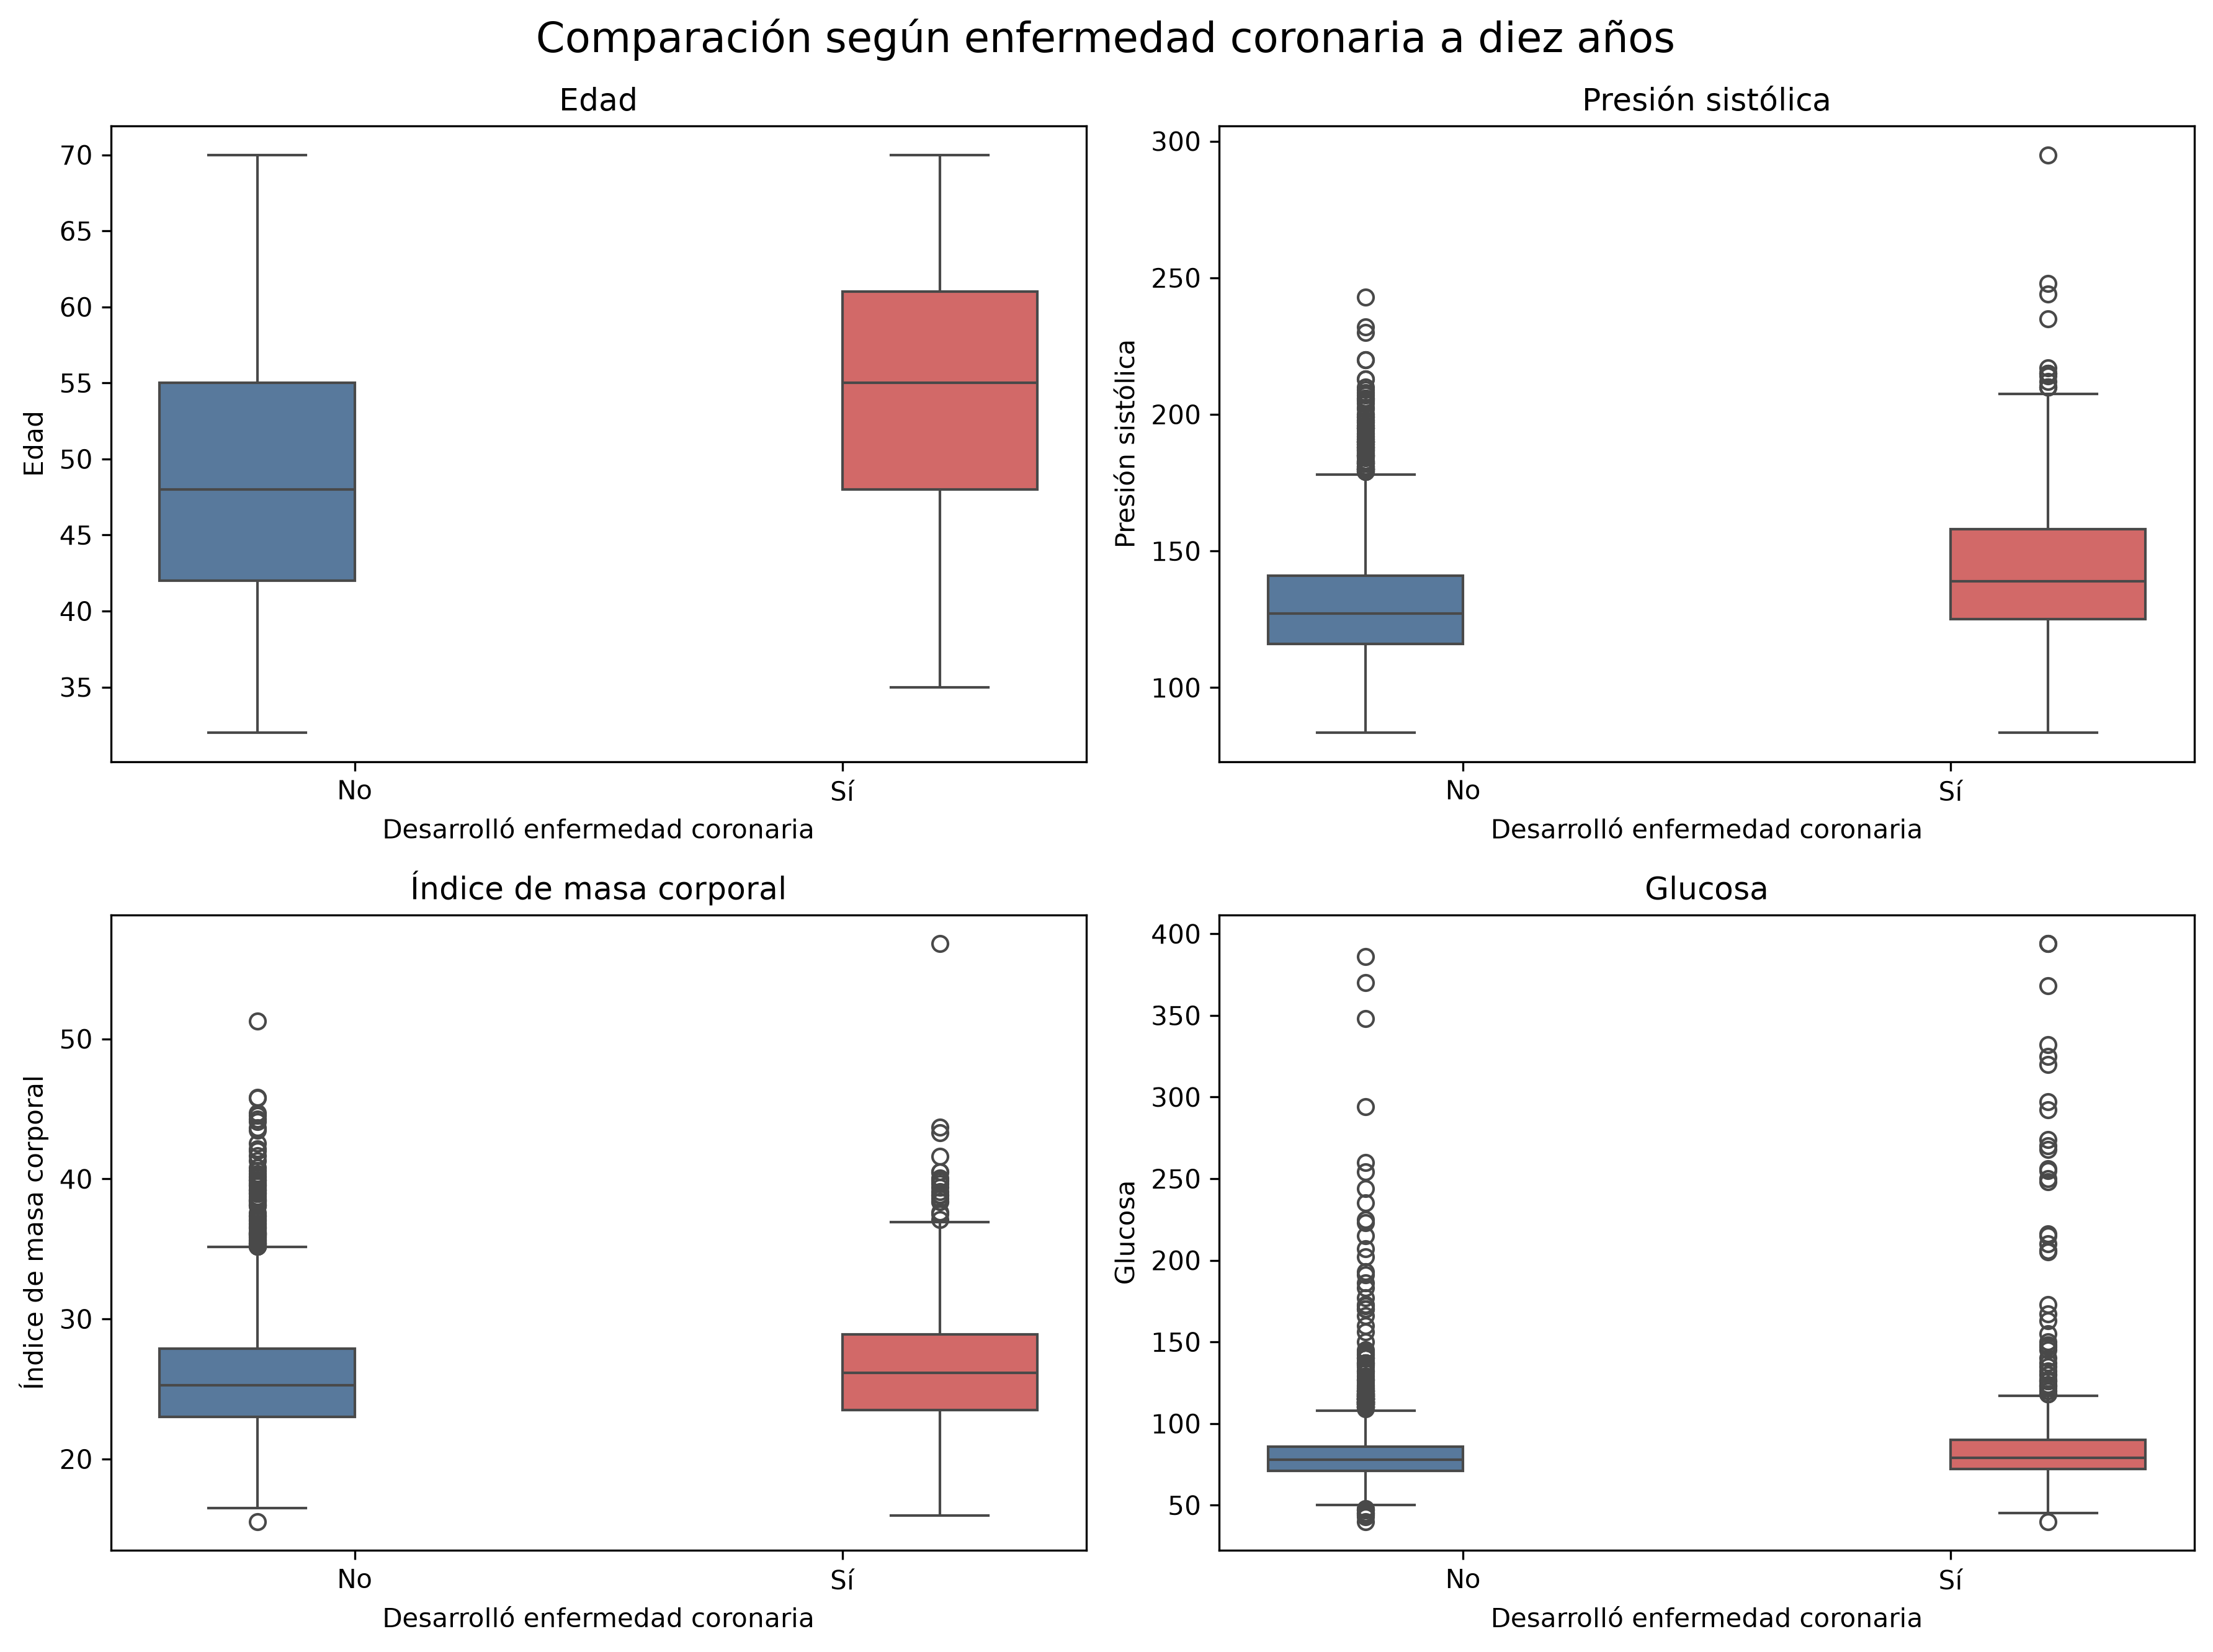
\includegraphics[width=0.86\textwidth]{../figuras/comparacion_variables_chd.png}
\caption{Comparación de edad, presión sistólica, índice de masa corporal y glucosa según enfermedad coronaria.}
\label{fig:comparacion}
\end{figure}

Como relación categórica preliminar, el 24,70\,\% de las personas con antecedente de hipertensión desarrolló enfermedad coronaria, frente al 10,92\,\% de quienes no presentaban dicho antecedente (Figura~\ref{fig:hipertension}). Esta comparación se conserva como hallazgo descriptivo y no se interpreta como efecto causal.

\begin{figure}[H]
\centering
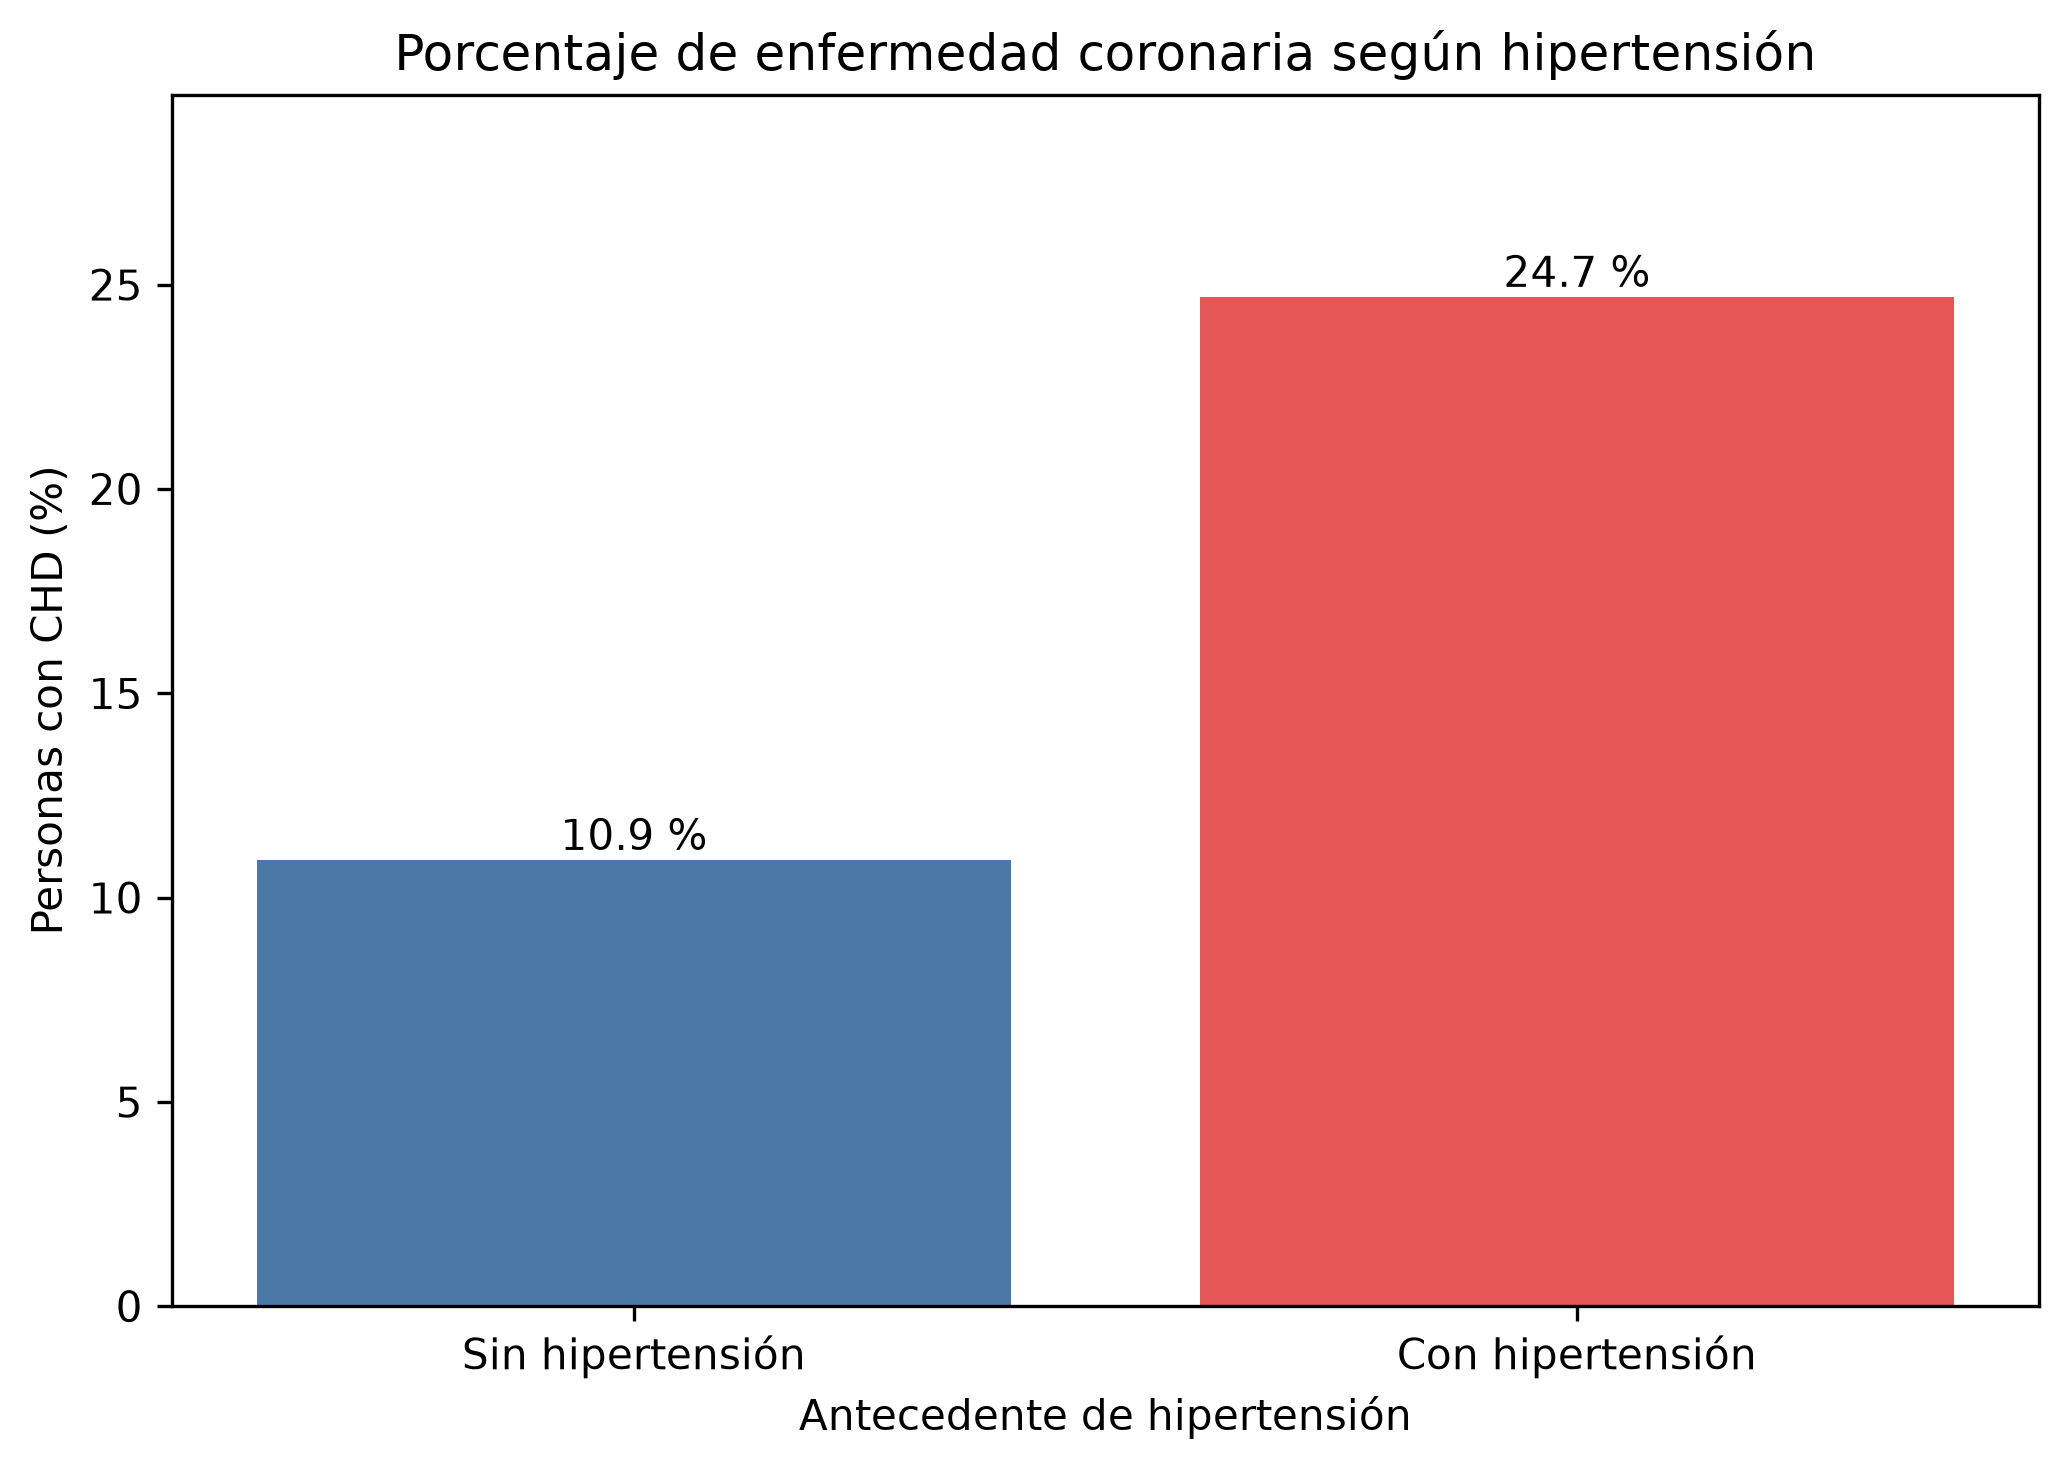
\includegraphics[width=0.62\textwidth]{../figuras/chd_segun_hipertension.png}
\caption{Porcentaje de enfermedad coronaria según antecedente de hipertensión.}
\label{fig:hipertension}
\end{figure}

% ===================== 3. Estimación ===============================
% Guía oficial de la plantilla (15 pts, ID1.3):
% Utilicen métodos de estimación puntual e intervalos de confianza para
% determinar parámetros poblacionales relevantes e interpreten los resultados.
\section{Estimación puntual e intervalos de confianza}

Se estimaron dos parámetros relevantes: la proporción de personas que desarrolló enfermedad coronaria y la media de presión arterial sistólica. En ambos casos se utilizó un nivel de confianza del 95\,\%.

\subsection{Proporción de enfermedad coronaria}

La estimación puntual fue $\hat{p}=644/4\,238=0,1520$. Para la proporción se aplicó el intervalo de Wilson, que evita depender exclusivamente de la aproximación normal simple y presenta un comportamiento adecuado para una respuesta binaria. El intervalo obtenido fue $[0,1415;\ 0,1631]$, es decir, entre 14,15\,\% y 16,31\,\%.

Este rango expresa la incertidumbre asociada a la estimación de la proporción poblacional bajo los supuestos del muestreo. No debe interpretarse como la probabilidad individual de cada persona ni como garantía de representatividad para poblaciones diferentes de la estudiada.

\subsection{Media de presión arterial sistólica}

La presión sistólica media observada fue $\bar{x}=132,35$ mmHg, con desviación estándar $s=22,04$ mmHg y error estándar $EE=0,34$ mmHg. Como la desviación estándar poblacional es desconocida, se utilizó un intervalo basado en la distribución $t$ de Student:

\[
\bar{x}\ \pm\ t_{0,975;n-1}\frac{s}{\sqrt{n}}.
\]

El intervalo de confianza del 95\,\% fue $[131,69;\ 133,02]$ mmHg. Su amplitud reducida refleja la precisión derivada del tamaño muestral, pero no implica que el 95\,\% de las mediciones individuales se encuentre dentro de ese rango. La Tabla~\ref{tab:intervalos} sintetiza ambas estimaciones.

\begin{table}[H]
\centering
\caption{Estimaciones puntuales e intervalos de confianza del 95\,\%.}
\label{tab:intervalos}
\small
\begin{tabular}{lrrr}
\toprule
\textbf{Parámetro} & \textbf{$n$} & \textbf{Estimación} & \textbf{IC 95\,\%} \\
\midrule
Proporción de enfermedad coronaria & 4.238 & 15,20\,\% & 14,15\,\%--16,31\,\% \\
Media de presión sistólica         & 4.238 & 132,35 mmHg & 131,69--133,02 mmHg \\
\bottomrule
\end{tabular}
\end{table}

% ===================== 4. Hipótesis ================================
% Guía oficial de la plantilla (15 pts, ID1.4):
% Apliquen al menos una prueba de hipótesis básica, seleccionando el
% procedimiento según el tipo de variable y el nivel de significancia.
\section{Aplicación de una prueba de hipótesis}

La comparación gráfica sugirió diferencias de presión sistólica entre las personas que desarrollaron enfermedad coronaria y aquellas que no la desarrollaron. Para evaluar formalmente esta diferencia se aplicó una prueba $t$ de Welch para dos muestras independientes. Esta variante es apropiada porque la variable de interés es cuantitativa y no exige igualdad de varianzas entre grupos.

Las hipótesis se definieron como:

\[
H_0:\ \mu_{\mathrm{CHD}}=\mu_{\mathrm{sin\ CHD}},
\qquad
H_1:\ \mu_{\mathrm{CHD}}\neq\mu_{\mathrm{sin\ CHD}}.
\]

Se estableció un nivel de significancia $\alpha=0,05$. La independencia entre personas depende del diseño del estudio y no puede verificarse solo con el archivo analizado. Los diagramas de caja muestran observaciones extremas, pero los tamaños de ambos grupos son grandes ($n_0=3.594$ y $n_1=644$), lo que aporta robustez al contraste de medias. La prueba de Welch evita imponer homogeneidad de varianzas.

\begin{table}[H]
\centering
\caption{Presión sistólica según ocurrencia de enfermedad coronaria.}
\label{tab:welch}
\small
\begin{tabular}{lrrr}
\toprule
\textbf{Grupo} & \textbf{$n$} & \textbf{Media (mmHg)} & \textbf{DE (mmHg)} \\
\midrule
Sin enfermedad coronaria & 3.594 & 130,33 & 20,46 \\
Con enfermedad coronaria & 644   & 143,62 & 26,69 \\
\bottomrule
\end{tabular}
\end{table}

La diferencia estimada, calculada como grupo con enfermedad menos grupo sin enfermedad, fue 13,29 mmHg. Su intervalo de confianza del 95\,\% fue $[11,11;\ 15,46]$ mmHg. La prueba produjo $t=12,015$ y $p<0,001$; por consiguiente, se rechazó $H_0$ y se concluyó que existe evidencia estadística de una diferencia en la presión sistólica media entre los grupos. El tamaño del efecto fue $d=0,617$, magnitud moderada que complementa la significancia estadística con una medida de relevancia práctica.

La conclusión se refiere a una asociación no ajustada. No demuestra que una mayor presión sistólica cause por sí sola la enfermedad coronaria, pues no se controlaron simultáneamente edad, sexo, tabaquismo, diabetes u otros posibles factores de confusión.

% ===================== 5. Documentación ============================
% Guía oficial de la plantilla (15 pts):
% Documenten clara, ordenada y completamente los procedimientos y resultados,
% de modo que el análisis sea trazable.
\section{Documentación de procedimientos y resultados}

El análisis se desarrolló en Python mediante un notebook de Jupyter y se organizó para mantener trazabilidad entre datos, código, resultados y figuras. El flujo aplicado fue el siguiente:

\begin{enumerate}[leftmargin=1.7em,itemsep=0.25em]
  \item Se conservó el archivo original \path{fase-1/datos/raw/framingham.csv} sin modificaciones.
  \item Se verificaron dimensiones, tipos computacionales, valores únicos, datos ausentes y filas duplicadas.
  \item Se creó una copia en memoria denominada \texttt{df\_analisis}; las variables binarias se trataron como nominales y \texttt{education} como ordinal.
  \item Se calcularon medidas descriptivas sobre los casos disponibles. No se imputaron valores ausentes durante esta etapa.
  \item Se exportaron las figuras con resolución de 300 dpi a \path{fase-1/formativa-1/figuras/}.
  \item Se construyeron intervalos de confianza del 95\,\% y se aplicó una prueba $t$ de Welch bilateral con $\alpha=0,05$.
\end{enumerate}

El notebook reproducible se denomina \texttt{formativa\_1\_framingham.ipynb} y se encuentra en \path{fase-1/formativa-1/notebooks/}. Las dependencias se registran en \path{requirements.txt}; entre las bibliotecas principales se encuentran pandas, NumPy, SciPy, statsmodels, Matplotlib y Seaborn. El repositorio completo está disponible en \proyRepo.

% ===================== 6. Interpretación ===========================
% Guía oficial de la plantilla (15 pts):
% Presenten interpretaciones preliminares claras y coherentes, vinculadas con
% el problema de decisión bajo incertidumbre.
\section{Interpretación preliminar de resultados}

El análisis muestra que 15,20\,\% de la muestra desarrolló enfermedad coronaria durante los diez años de seguimiento. La edad y la presión sistólica presentan las diferencias visuales más claras entre los grupos. En particular, la presión sistólica media fue 13,29 mmHg mayor entre quienes presentaron el evento, diferencia que resultó estadísticamente significativa y de magnitud moderada.

Desde una perspectiva de decisión bajo incertidumbre, los intervalos de confianza permiten distinguir entre el valor observado en la muestra y un rango plausible para el parámetro poblacional. La prueba de hipótesis agrega evidencia respecto de la diferencia de medias, mientras que el tamaño del efecto evita reducir la conclusión a la sola comparación del valor $p$ con $\alpha$.

Los resultados sugieren que la presión arterial y el antecedente de hipertensión son variables relevantes para profundizar el estudio cardiovascular. Sin embargo, una decisión clínica no debería basarse en una sola variable ni en comparaciones bivariadas. La interpretación requiere considerar conjuntamente características demográficas, conductuales y clínicas.

\subsection{Limitaciones}

El estudio es observacional y los análisis realizados no controlan factores de confusión; por ello, las asociaciones no permiten establecer causalidad. La representatividad de las estimaciones depende del diseño y de la población original del estudio Framingham. Además, siete variables contienen datos ausentes, con 9,16\,\% en glucosa. El análisis por casos disponibles conserva información, pero podría introducir sesgo si la ausencia no fuera aleatoria.

Las categorías poco frecuentes, como accidente cerebrovascular, diabetes y uso de medicamentos antihipertensivos, requieren cautela en comparaciones posteriores. Asimismo, el desequilibrio de la variable de respuesta debe considerarse si en fases siguientes se construyen modelos predictivos.

\subsection{Conclusiones y proyección}

La evaluación permitió definir el problema, documentar el conjunto de datos y clasificar correctamente sus variables. La estadística descriptiva identificó asimetrías, valores extremos y relaciones preliminares coherentes con el contexto cardiovascular. La estimación cuantificó la incertidumbre de la proporción de enfermedad coronaria y de la presión sistólica media, mientras que la prueba de Welch respaldó una diferencia entre los grupos con y sin enfermedad.

Como continuación del proyecto se propone evaluar el tratamiento de los datos ausentes, estudiar relaciones multivariadas y analizar la capacidad predictiva conjunta de las variables. En esas etapas se mantendrá la distinción entre descripción, asociación, predicción y causalidad.

% ===================== Control formal de entrega ===================
% Este criterio de la plantilla es una instrucción de revisión y no una sección
% de contenido. Antes de entregar se debe verificar: redacción formal, lenguaje
% estadístico adecuado, formato solicitado y versión final del PDF en Canvas.

% ===================== Referencias =================================
\begin{thebibliography}{9}
\raggedright

\bibitem{dileep}
Dileep, A. (2019).
\textit{Logistic Regression to Predict Heart Disease}.
Kaggle.
\url{https://www.kaggle.com/datasets/dileep070/heart-disease-prediction-using-logistic-regression}

\bibitem{nhlbi}
National Heart, Lung, and Blood Institute.
\textit{Teaching Datasets: Framingham Heart Study}.
\url{https://biolincc.nhlbi.nih.gov/teaching/}

\end{thebibliography}

\end{document}

